\chapter{What is ASP.Net}

\section{The .Net Platform}
.NET is a developer platform made up of tools, programming languages, and libraries for building many different types of applications.

The base platform provides components that apply to all different types of apps. Additional frameworks, such as ASP.NET, extend .NET with components for building specific types of apps.

Here are some things included in the .NET platform:
\begin{itemize}
	\tightlist
	\item The \textbf{C\#}, \textbf{F\#}, and \textbf{Visual Basic} programming languages
	\item \textbf{Base libraries} for working with strings, dates, files/IO, and more
	\item \textbf{Editors and tools} for Windows, Linux, macOS, and Docker
\end{itemize}

\section{ASP.NET extends .NET}
ASP.NET extends the .NET platform with tools and libraries specifically for building web apps.

These are some things that ASP.NET adds to the .NET platform:
\begin{itemize}
	\tightlist
	\item \textbf{Base framework} for processing web requests in C\# or F\#
	\item \textbf{Web-page templating syntax}, known as Razor, for building dynamic web pages using C\#
	\item \textbf{Libraries for common web patterns}, such as Model View Controller (MVC)
	\item \textbf{Authentication system} that includes libraries, a database, and template pages for handling logins, including multi-factor authentication and external authentication with Google, Twitter, and more.
	\item \textbf{Editor extensions} to provide syntax highlighting, code completion, and other functionality specifically for developing web pages
\end{itemize}

\section{Dynamic pages using C\#, HTML, CSS, and JavaScript}
Razor provides a syntax for creating dynamic web pages using HTML and C\#. Your C\# code is evaluated on the server and the resulting HTML content is sent to the user.

Code that executes client-side is written in JavaScript. ASP.NET integrates with JavaScript frameworks and includes pre-configured templates for single page app (SPA) frameworks like React and Angular.

\begin{figure}[h]
	\centering
	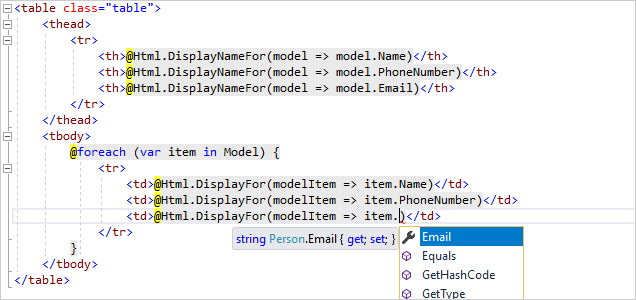
\includegraphics[width=0.85\linewidth]{img/a1}
	\caption{\textit{Dynamic Pages in ASP.Net}}
	\label{fig:asp_dynamic}
\end{figure}


\chapter{ASP.Net Master Pages}

\section{Introduction}
ASP.NET master pages allow you to create a consistent layout for the pages in your application. A single master page defines the look and feel and standard behavior that you want for all of the pages (or a group of pages) in your application. You can then create individual content pages that contain the content you want to display. When users request the content pages, they merge with the master page to produce output that combines the layout of the master page with the content from the content page.

\section{How Master Pages Work}
Master pages actually consist of two pieces, the master page itself and one or more content pages.
\subsection{Master Pages}
A master page is an ASP.NET file with the extension .master (for example, MySite.master) with a predefined layout that can include static text, HTML elements, and server controls. The master page is identified by a special @ Master directive that replaces the @ Page directive that is used for ordinary .aspx pages. The directive looks like the following.
\begin{lstlisting}
<%@ Master Language="C#" %>
\end{lstlisting}
In addition to the @ Master directive, the master page also contains all of the top-level HTML elements for a page, such as html, head, and form. For example, on a master page you might use an HTML table for the layout, an img element for your company logo, static text for the copyright notice, and server controls to create standard navigation for your site. You can use any HTML and any ASP.NET elements as part of your master page.
\begin{lstlisting}
<%@ Master Language="C#" CodeFile="MasterPage.master.cs" Inherits="MasterPage" %>
\end{lstlisting}
In addition to the @ Master directive, the master page also contains all of the top-level HTML elements for a page, such as html, head, and form. For example, on a master page you might use an HTML table for the layout, an img element for your company logo, static text for the copyright notice, and server controls to create standard navigation for your site. You can use any HTML and any ASP.NET elements as part of your master page.

\subsection{Replaceable Content Placeholders}
In addition to static text and controls that will appear on all pages, the master page also includes one or more ContentPlaceHolder controls. These placeholder controls define regions where replaceable content will appear. In turn, the replaceable content is defined in content pages. After you have defined the ContentPlaceHolder controls, a master page might look like the following.
\begin{lstlisting}
<% @ Master Language="C#" %>

<!DOCTYPE html PUBLIC "-//W3C//DTD XHTML 
	1.1//EN" "http://www.w3.org/TR/xhtml11/DTD/xhtml11.dtd">

<html xmlns="http://www.w3.org/1999/xhtml" >
	<head runat="server" >
		<title>Master page title</title>
	</head>
	<body>
		<form id="form1" runat="server">
			<table>
				<tr>
					<td><asp:contentplaceholder id="Main" runat="server" /></td>
					<td><asp:contentplaceholder id="Footer" runat="server" /></td>
				</tr>
			</table>
		</form>
	</body>
</html>
\end{lstlisting}

\subsection{Content Pages}
You define the content for the master page's placeholder controls by creating individual content pages, which are ASP.NET pages (.aspx files and, optionally, code-behind files) that are bound to a specific master page. The binding is established in the content page's @ Page directive by including a MasterPageFile attribute that points to the master page to be used. For example, a content page might have the following @ Page directive, which binds it to the Master1.master page.
\begin{lstlisting}
<%@ Page Language="C#" MasterPageFile="~/MasterPages/Master1.master" Title="Content Page" %>
\end{lstlisting}
In the content page, you create the content by adding Content controls and mapping them to ContentPlaceHolder controls on the master page. For example, the master page might have content placeholders called Main and Footer. In the content page, you can create two Content controls, one that is mapped to the ContentPlaceHolder control Main and the other mapped to the ContentPlaceHolder control Footer, as shown in the following figure.

After creating Content controls, you add text and controls to them. In a content page, anything that is not inside the Content controls (except script blocks for server code) results in an error. You can perform any tasks in a content page that you do in an ASP.NET page. For example, you can generate content for a Content control using server controls and database queries or other dynamic mechanisms.

A content page might look like the following.
\begin{lstlisting}
<% @ Page Language="C#" MasterPageFile="~/Master.master" Title="Content Page 1" %>
<asp:Content ID="Content1" ContentPlaceHolderID="Main" Runat="Server">
	Main content.
</asp:Content>

<asp:Content ID="Content2" ContentPlaceHolderID="Footer" Runat="Server" >
	Footer content.
</asp:content>
\end{lstlisting}
The @ Page directive binds the content page to a specific master page, and it defines a title for the page that will be merged into the master page. Note that the content page contains no other markup outside of the Content controls. (The master page must contain a head element with the attribute runat="server" so that the title setting can be merged at run time.)

You can create multiple master pages to define different layouts for different parts of your site, and a different set of content pages for each master page.

\section{Advantages of Master Pages}
Master pages provide functionality that developers have traditionally created by copying existing code, text, and control elements repeatedly; using framesets; using include files for common elements; using ASP.NET user controls; and so on. Advantages of master pages include the following:
\begin{itemize}
	\tightlist
	\item They allow you to centralize the common functionality of your pages so that you can make updates in just one place.	
	\item They make it easy to create one set of controls and code and apply the results to a set of pages. For example, you can use controls on the master page to create a menu that applies to all pages.	
	\item They give you fine-grained control over the layout of the final page by allowing you to control how the placeholder controls are rendered.	
	\item They provide an object model that allows you to customize the master page from individual content pages.
\end{itemize}

\section{Run-time Behavior of Master Pages}
At run time, master pages are handled in the following sequence:
\begin{enumerate}
	\tightlist
	\item Users request a page by typing the URL of the content page.	
	\item When the page is fetched, the @ Page directive is read. If the directive references a master page, the master page is read as well. If this is the first time the pages have been requested, both pages are compiled.	
	\item The master page with the updated content is merged into the control tree of the content page.	
	\item The content of individual Content controls is merged into the corresponding ContentPlaceHolder control in the master page.	
	\item The resulting merged page is rendered to the browser.
\end{enumerate}
From the user's perspective, the combined master and content pages are a single, discrete page. The URL of the page is that of the content page.

From a programming perspective, the two pages act as separate containers for their respective controls. The content page acts as a container for the master page. However, you can reference public master-page members from code in the content page, as described in the next section.

Note that the master page becomes a part of the content page. In effect, the master page acts in much the same way a user control acts — as a child of the content page and as a container within that page. In this case, however, the master page is the container for all of the server controls that are rendered to the browser. The control tree for a merged master and content page looks something like this:
\begin{lstlisting}
Page
	Master Page
		(Master page markup and controls)
		ContentPlaceHolder
			Content page markup and server controls
		(Master page markup and controls)
		ContentPlaceHolder
			Content page markup and server controls
		(Master page markup and controls)
\end{lstlisting}
This diagram is simplified; if the content page does not have corresponding Content controls, the master page might also have markup and controls in the ContentPlaceHolder controls.

In general, this structure has no effect on how you construct your pages or program them. However, in some cases, if you set a page-wide property on the master page, it can affect the behavior of the content page, because the master page is the closest parent for the controls on the page. For example, if you set the EnableViewState property on the content page to true but set the same property to false in the master page, view state will effectively be disabled because the setting on the master page will take priority.

\section{Master Pages and Themes}
You cannot directly apply an ASP.NET theme to a master page. If you add a theme attribute to the @ Master directive, the page will raise an error when it runs.

However, themes are applied to master pages under these circumstances:
\begin{itemize}
	\item If a theme is defined in the content page. Master pages are resolved in the context of content pages, so the content page's theme is applied to the master page as well.	
	\item If the site as a whole is configured to use a theme by including a theme definition in the pages Element (ASP.NET Settings Schema) element.
\end{itemize}


\chapter{Themes and Skins}
\section{Introduction}
A theme is a collection of property settings that allow you to define the look of pages and controls, and then apply the look consistently across pages in a Web application, across an entire Web application, or across all Web applications on a server.

\section{Themes and Control Skins}
Themes are made up of a set of elements: skins, cascading style sheets (CSS), images, and other resources. At a minimum, a theme will contain skins. Themes are defined in special directories in your Web site or on your Web server.

\subsection{Skins}
A skin file has the file name extension .skin and contains property settings for individual controls such as Button, Label, TextBox, or Calendar controls. Control skin settings are like the control markup itself, but contain only the properties you want to set as part of the theme. For example, the following is a control skin for a Button control:
\begin{lstlisting}
<asp:button runat="server" BackColor="lightblue" ForeColor="black" />
\end{lstlisting}
You create .skin files in the Theme folder. A .skin file can contain one or more control skins for one or more control types. You can define skins in a separate file for each control or define all the skins for a theme in a single file.
There are two types of control skins, default skins and named skins:
\begin{itemize}
	\item A default skin automatically applies to all controls of the same type when a theme is applied to a page. A control skin is a default skin if it does not have a SkinID attribute. For example, if you create a default skin for a Calendar control, the control skin applies to all Calendar controls on pages that use the theme. (Default skins are matched exactly by control type, so that a Button control skin applies to all Button controls, but not to LinkButton controls or to controls that derive from the Button object.)	
	\item A named skin is a control skin with a SkinID property set. Named skins do not automatically apply to controls by type. Instead, you explicitly apply a named skin to a control by setting the control's SkinID property. Creating named skins allows you to set different skins for different instances of the same control in an application.
\end{itemize}

\subsection{Cascading Style Sheets}
A theme can also include a cascading style sheet (.css file). When you put a .css file in the theme folder, the style sheet is applied automatically as part of the theme. You define a style sheet using the file name extension .css in the theme folder.

\subsection{Theme Graphics and Other Resources}
Themes can also include graphics and other resources, such as script files or sound files. For example, part of your page theme might include a skin for a TreeView control. As part of the theme, you can include the graphics used to represent the expand button and the collapse button.

Typically, the resource files for the theme are in the same folder as the skin files for that theme, but they can be elsewhere in the Web application, in a subfolder of the theme folder for example. To refer to a resource file in a subfolder of the theme folder, use a path like the one shown in this Image control skin:
\begin{lstlisting}
<asp:Image runat="server" ImageUrl="ThemeSubfolder/filename.ext" />
\end{lstlisting}
You can also store your resource files outside the theme folder. If you use the tilde (~) syntax to refer to the resource files, the Web application will automatically find the images. For example, if you place the resources for a theme in a subfolder of your application, you can use paths of the form ~/SubFolder/filename.ext to refer to resource files, as in the following example.
\begin{lstlisting}
<asp:Image runat="server" ImageUrl="~/AppSubfolder/filename.ext" />
\end{lstlisting}

\section{Scoping Themes}
You can define themes for a single Web application, or as global themes that can be used by all applications on a Web server. After a theme is defined, it can be placed on individual pages using the Theme or StyleSheetTheme attribute of the @ Page directive, or it can be applied to all pages in an application by setting the <pages> element in the application configuration file. If the <pages> element is defined in the Machine.config file, the theme will apply to all pages in Web applications on the server.

\subsection{Page Themes}
A page theme is a theme folder with control skins, style sheets, graphics files and other resources created as a subfolder of the \\App\_Themes folder in your Web site. Each theme is a different subfolder of the \\App\_Themes folder. The following example shows a typical page theme, defining two themes named BlueTheme and PinkTheme.
\begin{lstlisting}
MyWebSite
	App_Themes
		BlueTheme
			Controls.skin
			BlueTheme.css
		PinkTheme
			Controls.skin
			PinkTheme.css
\end{lstlisting}

\subsection{Global Themes}
A global theme is a theme that you can apply to all the Web sites on a server. Global themes allow you to define an overall look for your domain when you maintain multiple Web sites on the same server.

Global themes are like page themes in that they include property settings, style sheet settings, and graphics. However, global themes are stored in a folder named Themes that is global to the Web server. Any Web site on the server, and any page in any Web site, can reference a global theme.

\section{Theme Settings Precedence}
You can specify the precedence that theme settings take over local control settings by specifying how the theme is applied.

If you set a page's Theme property, control settings in the theme and the page are merged to form the final settings for the control. If a control setting is defined in both the control and the theme, the control settings from the theme override any page settings on the control. This strategy enables the theme to create a consistent look across pages, even if controls on the pages already have individual property settings. For example, it allows you to apply a theme to a page you created in an earlier version of ASP.NET.

Alternatively, you can apply a theme as a style sheet theme by setting the page's StyleSheetTheme property. In this case, local page settings take precedence over those defined in the theme when the setting is defined in both places. This is the model used by cascading style sheets. You might apply a theme as a style sheet theme if you want to be able to set the properties of individual controls on the page while still applying a theme for an overall look.

Global theme elements cannot be partially replaced by elements of application-level themes. If you create an application-level theme with the same name as a global theme, theme elements in the application-level theme will not override the global theme elements.

\section{Properties You Can Define Using Themes}
As a rule, you can use themes to define properties that concern a page or control's appearance or static content. You can set only those properties that have a ThemeableAttribute attribute set to true in the control class.

Properties that explicitly specify control behavior rather than appearance do not accept theme values. For example, you cannot set a Button control's CommandName property by using a theme. Similarly, you cannot use a theme to set a GridView control's AllowPaging property or DataSource property.

Note that you cannot use expression builders, which generate code expressions for assignment in a page at compile time, in themes or skins.

\section{Themes vs. Cascading Style Sheets}
Themes are similar to cascading style sheets in that both themes and style sheets define a set of common attributes that can be applied to any page. However, themes differ from style sheets in the following ways:
\begin{itemize}
	\item Themes can define many properties of a control or page, not just style properties. For example, using themes, you can specify the graphics for a TreeView control, the template layout of a GridView control, and so on.	
	\item Themes can include graphics.	
	\item Themes do not cascade the way style sheets do. By default, any property values defined in a theme referenced by a page's Theme property override the property values declaratively set on a control, unless you explicitly apply the theme using the StyleSheetTheme property. For more information, see the Theme Settings Precedence section above.	
	\item Only one theme can be applied to each page. You cannot apply multiple themes to a page, unlike style sheets where multiple style sheets can be applied.
\end{itemize}

\section{Security Considerations}
Themes can cause security issues when they are used on your Web site. Malicious themes can be used to:
\begin{itemize}
	\item Alter a control's behavior so that it does not behave as expected.	
	\item Inject client-side script, therefore posing a cross-site scripting risk.	
	\item Alter validation.	
	\item Expose sensitive information.	
	\item The mitigations for these common threats are:	
	\item Protect the global and application theme directories with proper access control settings. Only trusted users should be allowed to write files to the theme directories.	
	\item Do not use themes from an untrusted source. Always examine any themes from outside your organization for malicious code before using them on you Web site.	
	\item Do not expose the theme name in query data. Malicious users could use this information to use themes that are unknown to the developer and thereby expose sensitive information.
\end{itemize}


\chapter{Examples}

Consider the following Master Page: 
\begin{figure}[h]
	\centering
	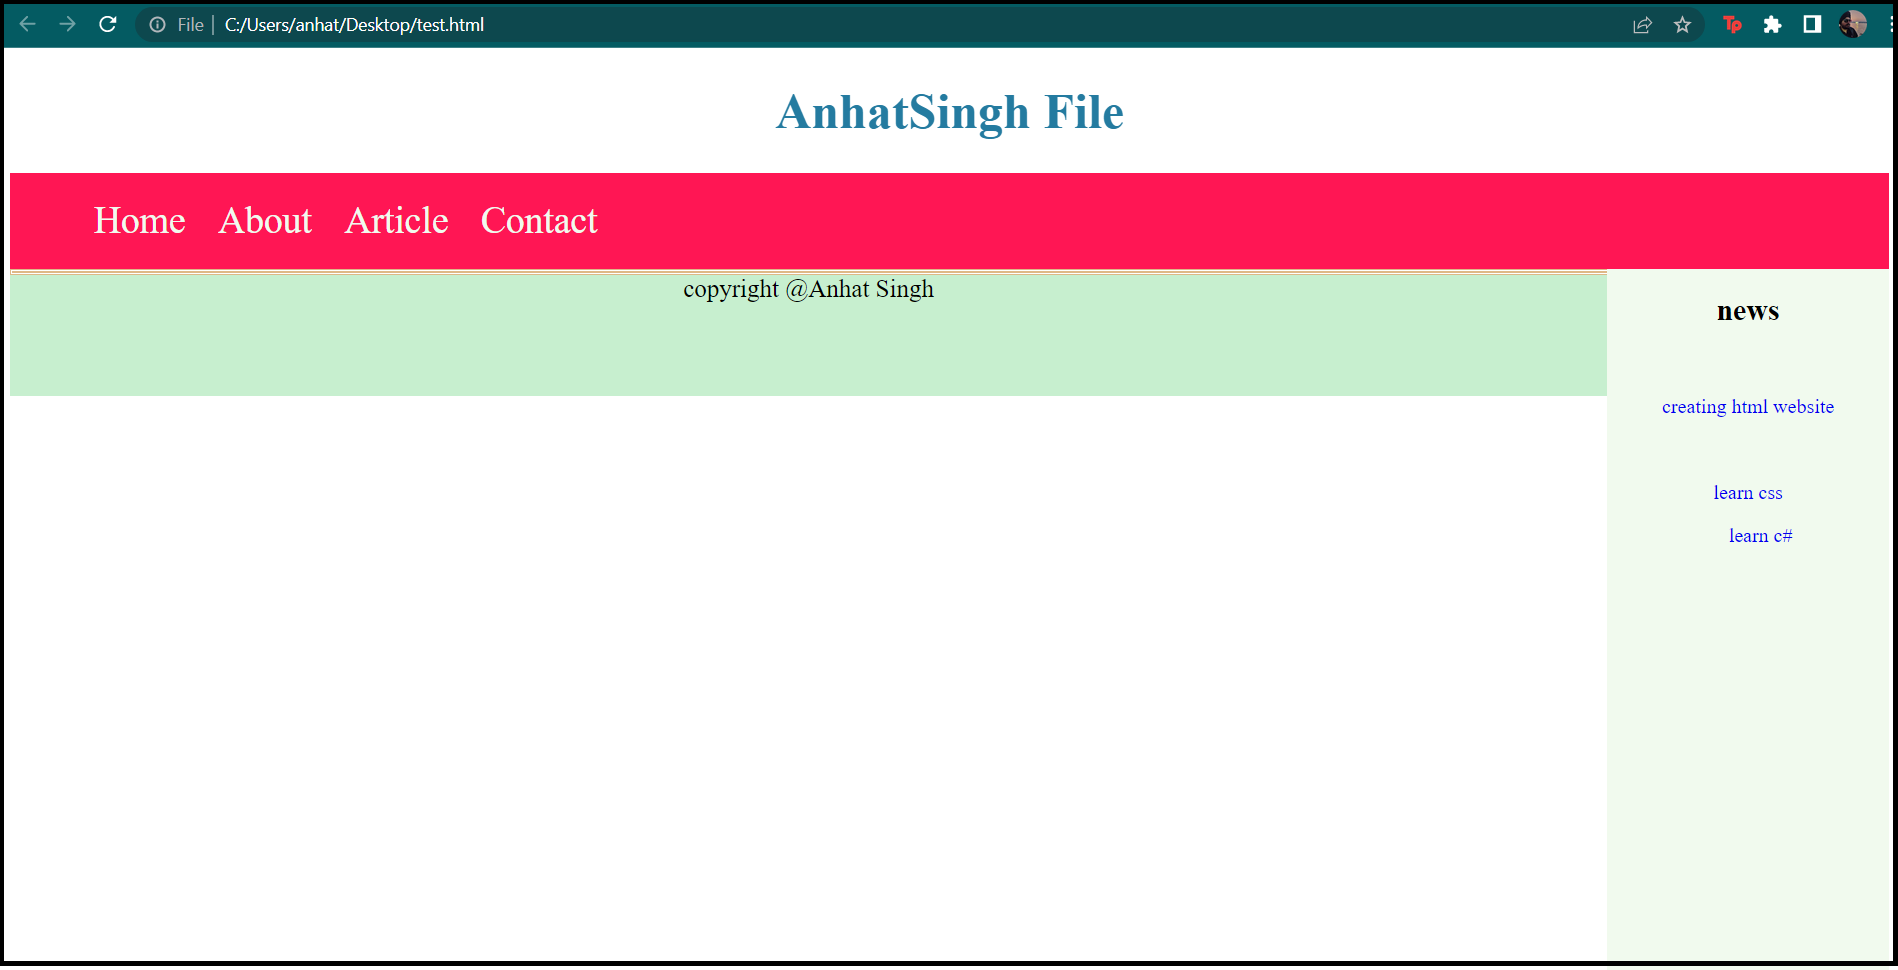
\includegraphics[width=0.95\linewidth]{img/a3}
	\caption{\textit{Master Page in ASP.Net}}
	\label{fig:masterPage}
\end{figure}

\begin{lstlisting}[language=html,caption={Master Page Code},captionpos=t]
<%@ Master Language="C#" AutoEventWireup="true" CodeBehind="Site1.master.cs" Inherits="masterpage.Site1" %>  
<!DOCTYPE html>  
<html xmlns="http://www.w3.org/1999/xhtml">  
	<head runat="server">  
		<title>AnhatSingh</title>  
		<link href="css/my.css" rel="stylesheet" />  
		<asp:ContentPlaceHolder ID="head" runat="server">  
		</asp:ContentPlaceHolder>  
	</head>  
	<body>  
		<!DOCTYPE html>  
		<html>  
			<head>  
				<title>my layout</title>  
				<link rel="stylesheet" type="text/css" href="my.css">  
			</head>  
			<body>  
				<header id="header">  
					<h1>AnhatSingh File</h1>  
				</header>  
				<nav id="nav">  
					<ul>  
						<li><a href="home.aspx">Home</a></li>  
						<li><a href="#">About</a></li>  
						<li><a href="#">Article</a></li>  
						<li><a href="#">Contact</a></li>  
					</ul>  
				</nav>  
				<aside id="side">  
					<h1>news</h1>  
					<a href="#"><p>creating html website</p></a>  
					<a href="#"><p>learn css</p></a>  
					<a href="#">learn c#</a>  
				</aside>  
				<div id="con">  
					<asp:ContentPlaceHolder ID="ContentPlaceHolder1" runat="server">  
					</asp:ContentPlaceHolder>  
				</div>
				<footer id="footer">  
					copyright @Anhat Singh
				</footer>  
			</body>  
		</html>  
		<form id="form1" runat="server">  
		</form>
	</body>  
</html> 
\end{lstlisting}

\begin{lstlisting}[caption={CSS Code},captionpos=t]
#header{  
	color: #247BA0;  
	text-align: center;  
	font-size: 20px;  
}  
#nav{  
	background-color:#FF1654;  
	padding: 5px;  
}  
ul{  
	
	list-style-type: none;  
}  
li a {  
	color: #F1FAEE;  
	font-size: 30px;  
	column-width: 5%;  
}  
li  
{  
	display: inline;  
	padding-left: 2px;  
	column-width: 20px;  
}  
a{  
	text-decoration: none;  
	margin-left:20px  
}  
li a:hover{  
	background-color: #F3FFBD;  
	color: #FF1654;  
	padding:1%;  
}  
#side{  
	text-align: center;  
	float: right;  
	width: 15%;  
	padding-bottom: 79%;  
	background-color: #F1FAEE;  
}  
#article{  
	background-color: #EEF5DB;  
	padding: 10px;  
	padding-bottom: 75%;  
}  
#footer{  
	background-color: #C7EFCF;  
	text-align:center;  
	padding-bottom: 5%;  
	font-size: 20px;  
}  
#con{  
	border:double;  
	border-color:burlywood;  
}
\end{lstlisting}

\begin{lstlisting}[language=html,caption={Home.aspx},captionpos=t]
<%@ Page Title="" Language="C#" MasterPageFile="~/Site1.Master" AutoEventWireup="true" CodeBehind="home.aspx.cs" Inherits="masterpage.home" %>  
<asp:Content ID="Content1" ContentPlaceHolderID="head" runat="server">  
</asp:Content>  
<asp:Content ID="Content2" ContentPlaceHolderID="ContentPlaceHolder1" runat="server">  
	<h1>Home page</h1>  
</asp:Content>
\end{lstlisting}